Des travaux initiaux avaient été réalisés en Python par Samuel Charron. Il avait créé un plugin Python capable de récupérer des signaux depuis une API. N'étant pas formé au Python, j'ai préféré commencer mes travaux en utilisant le Java avec l'accord de Samuel. Je savais en m'orientant vers le Java, qu'une fois que l'application obtiendrait de bonnes performance, j'aurais à implémenter son fonctionnement général en Python sous forme de plugin.

\section{Démarche de travail}
    Ce projet s'inscrit parfaitement dans le type de projet R\&D. De ce fait, l'avancement est très difficile à planifier dans le temps. Surtout lorsque l'on ne connaît pas les différentes notions sous-jacentes au projet et qu'il y a une bonne part d'auto-formation avant de pouvoir développer une application.

    \subsection{Mes acquis à l'INSA}
        Les connaissances générales que j'avais en \textit{Data Science}, avant le début du stage, concernaient le \textit{Data Mining} en contexte \textbf{numérique} et étaient les suivantes :
        \begin{itemize}
            \item Concepts en analyse et normalisation de données : Analyse en Composantes Principales (ACP), centrage et réduction de données numériques ;
            \item Concepts d'apprentissage non-supervisé : méthodes de regroupement des données (Clustering : Classification Hiérarchique Ascendante, Algorithme des K-Means, Modèles de mélanges et Algorithmes EM) ;
            \item Base de l'optimisation : méthodes du gradient et de Newton, introduction aux outils mathématiques pour l'optimisation sous contraintes convexe ;
            \item Concepts d'apprentissage supervisé : méthodes pour la discrimination de données (Décision Bayésienne, Régression logistique, SVM linéaire) et notions de validation croisée.\\
        \end{itemize}

        Ce projet ne permet pas de mettre mes connaissances en apprentissage non-supervisé en avant. Cependant, mes notions d'apprentissage supervisé telles que : la démarche à suivre pour construire un classifieur, les concepts liées à la validation des performances (validation croisée) et la notion de sur-apprentissage ; ont été fort utiles.\\

        D'une manière générale, mes connaissances en \textit{Text Mining} n'étaient pas suffisamment étoffées pour pouvoir dire tel classifieur est plus performant qu'un autre dans tel contexte (binaire ou multi-classes). En effet, ma formation (à l'INSA) est axée manipulation et traitement de données en contexte \textbf{numérique}. De ce fait, la manipulation et le traitement de données textuelles m'étaient inconnus.\\

        Une formation en \textit{Text Mining} m'a donc été indispensable avant de pouvoir commencer à travailler.

    \subsection{Déroulement du stage}
        Ainsi, durant les deux premiers mois, j'ai exploré le domaine du \textit{Text Mining} et du \textit{Natural Language Processing} au travers de la bibliothèque de Stanford implémentée en Java (\textit{Stanford Natural Language Processing}). Conjointement, j'ai étudié les cours associés, et construit une première application Spring répondant aux contraintes évoquées en partie \ref{sec:ma_mission_chez_data_publica} (sauf le critère du langage). Le travail en ressortant est décrit en partie \ref{sec:travaux_realises_en_java}.\\

        Ensuite, lors du dernier mois, j’ai implémenté le comportement général de cette application sous la forme d’un plugin Python, visible en partie \ref{}. Certain composants n'existaient pas en Python, je les ai donc ré-implémenté.

\section{Travaux réalisés en Java}
\label{sec:travaux_realises_en_java}
    \subsection{Présentation de mon environnement de travail}
        Dans C-Radar tout les traitements de type \og computing \fg (calcul) sont réalisés en Python (cf partie \ref{subsub:archi_tech}). De ce fait, créer une application permettant de classifier les signaux, devrait être fait en Python sous la forme d'un plugin (comme le requiert ma mission). Ayant fait le choix de commencer mes recherches en Java, il a fallu m'initialiser un environnement de travail un peu différent de l'environnement de travail Python.\\

        \paragraph{Spring et MongoDB :}
            Ainsi, Loïc Petit m'a créé une application Spring de base permettant de me connecter en local à une base de données Mongo. L'application me fournit un environnement de travail dans lequel construire le classifier à partir des signaux validés. Les signaux eux-mêmes récupérés depuis une base de données Mongo. Cette base de données contient mon ensemble de signaux permettant de construire et tester mon classifier. Les 1426 signaux validés y sont stocké ainsi que 350.000 autres signaux non validés (voir le dernier paragraphe de la partie \ref{sec:etat_bd}).\\

        Voici comment les signaux sont stockés dans Mongo :
\begin{verbatim}
{
    "id" : "TWITTER:agencenetdesign:329129810423083009",
    "content" : "Salon eCom Genève : l'équipe ND est en place au stand E1 \:) #ecomSITB http://t.co/YtsEs6rcDR",
    "publicationDate" : ISODate(2013-04-30T07:07:16Z),
    "sourceId" : "TWITTER:agencenetdesign",
    "source" : {
        "type" : "TWITTER",
        "resourceId" : "agencenetdesign"
    },
    "externalSignalId" : 329129810423083009,
    "validated" : false,
    "validatedTags" : [ ],
    "tags" : [
        "EVENT"
    ],
    "url" : "http://twitter.com/agencenetdesign/status/329129810423083009"
}
\end{verbatim}

        Le signal comporte :
        \begin{itemize}
            \item un identifieur unique \textit{id} ;
            \item un contenu \textit{content} ;
            \item une date de publication \textit{publicationDate} ;
            \item l'identifieur de la source \textit{sourceId} ;
            \item la source \textit{source} composé :
            \begin{itemize}
                \item du type de réseau dont provient le signal \textit{type} ;
                \item de l'identifieur du publieur dans ce réseau \textit{resourceId} ;
            \end{itemize}
            \item un identifeur externe \textit{externalSignalId} ;
            \item un booléen spécifiant si le signal a été manuellement validé ou non \textit{validated} ;
            \item la liste des tags s'il a été validé \textit{validatedTags}, la liste des tags potentiels (trouvés par le classifieur) \textit{tags} ;
            \item l'url là où a été publié le signal \textit{url}.
        \end{itemize}

        \paragraph{Formation Spring et Mongo :}
            Je me suis rapidement formé à Spring et Mongo pour pouvoir interfacer ces deux composants ensemble. Pour cela, j'ai suivi les tutoriels de Spring disponibles sur \href{https://spring.io/guides/gs/accessing-data-mongodb/}{https://spring.io/guides/gs/accessing-data-mongodb/}.\\
            Grâce aux tutoriels, j'ai appris à créer mes premiers points d'API permettant de faire des requêtes dans Mongo. Ces requêtes sont relativement basiques : récupérer tout les signaux sous forme de liste, récupérer uniquement les signaux validés (également sous forme de liste), savoir combien de signaux sont stockés dans ma base, etc. J'ai appris à faire ce type de requête dans Mongo grâce à la documentation sur \href{https://docs.mongodb.org/manual/}{https://docs.mongodb.org/manual/}. Les concepts de base de Mongo ne sont pas très compliqués à comprendre quand on a des notions de base de données.\\

    \subsection{Le \textit{Text Mining} et le \textit{Natural Language Processing} avec la bibliothèque de Stanford}
        Dès que j'ai été capable de faire ce type de requêtes auprès de ma base de données, il fallait à présent me concentrer sur le traitement des signaux, et donc la construction du classifieur. C'est à ce moment que je me suis intéressé à la bibliothèque de Stanford.

        \subsubsection{La bibliothèque : Stanford Natural Language Processing}
            Samuel Charron avait connaissance de l'existence de cette bibliothèque. De ce fait, il m'a conseillé de me former en \textit{Text Mining} et en \textit{Natural Language Processing} au travers de celle-ci puisqu'elle est implémentée en Java. Je me suis donc plongé dedans afin de découvrir les diverses fonctionnalités qu'elle propose. Celle-ci propose un ensemble d'outils pour le traitement automatique du langage naturel de la langue anglaise, chinoise et espagnole. Voici ces différents outils :

            \paragraph{Stanford POS Tagger (Part-Of-Speech) :}
                Le \textit{POS Tagger} permet de savoir la fonction grammaticale de chaque mot d'une phrase. Celui-ci fonctionne aussi pour le français.\\
                \textbf{Exemple :}
\begin{lstlisting}
K$\overbrace{Gustave}^{\highlight[cyan]{NNP}} \overbrace{is}^{\highlight[green]{VBZ}} \overbrace{the}^{\highlight[magenta]{DT}} \overbrace{firstname}^{\highlight[cyan]{NN}} \overbrace{of}^{\highlight[yellow]{IN}} \overbrace{a}^{\highlight[magenta]{DT}} \overbrace{very}^{\highlight[yellow]{RB}} \overbrace{famous}^{\highlight[yellow]{JJ}} \overbrace{french}^{\highlight[yellow]{JJ}} \overbrace{architect}^{\highlight[cyan]{NN}}\overbrace{.}^{\highlight[gray]{.}}$W
\end{lstlisting}
            \paragraph{Stanford Parser :}
                Le \textit{Parser} permet de connaître la structure grammaticale d'une phrase, à savoir quel(s) groupe(s) de mots forme(nt) le sujet, quel(s) groupe(s) de mots forme(nt) le verbe et quel(s) groupe(s) de mots forme(nt) le complément. Cet outils est une sur-couche du \textit{POS Tagger}. En effet, il réutilise, entre autres, son résultat pour en déduire la structure grammaticale d'une phrase.\\
                \textbf{Exemple :}\\
                Entrée : \og My internship was a rewarding experience.\fg\\
                Sortie :
\begin{lstlisting}
K(\textcolor{blue}{ROOT}W
  K(\textcolor{blue}{S}W
    K(\textcolor{blue}{NP} (\textcolor{gray}{PRP}\$ My) (\textcolor{cyan}{NN} internship))W
    K(\textcolor{blue}{VP} (\textcolor{green}{VBD} was)W
      K(\textcolor{blue}{NP} (\textcolor{magenta}{DT} a) (\textcolor{yellow}{JJ} rewarding) (\textcolor{cyan}{NN} experience))W
    K(\textcolor{cyan}{.} .)))W
\end{lstlisting}

            \paragraph{Stanford Named Entity Recognizer :}
                Le \textit{Named Entity Recognizer} permet d'identifier les groupes de mots qui sont des noms de personne, d'entreprises, de gènes, etc.
                \textbf{Exemple :}

            \paragraph{Stanford Classifier :}
                Le \textit{Classifier} permet de construire un classifieur automatique pour la catégorisation de texte.
                \textbf{Exemple :}

            \paragraph{Stanford Deterministic Coreference Resolution System :}
                Le \textit{Deterministic Coreference Resolution System} permet de trouver les expressions qui font référence à une même entité.
                \textbf{Exemple :}

            \paragraph{Stanford CoreNLP :}
                Le \textit{CoreNLP} permet de construire une suite de traitements automatiques (les traitements précédents) sur de l'anglais, du chinois, de l'espagnol. Un exemple de chaîne de traitement est visible en figure \ref{fig:coreNLP}.

            \begin{figure}[h!]
                \centering
                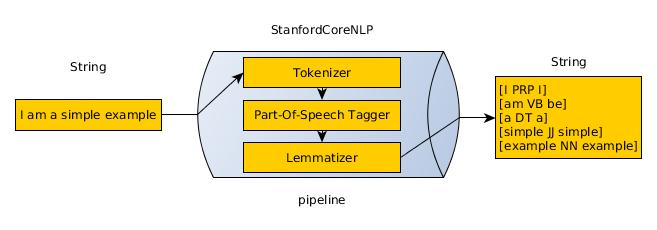
\includegraphics[width=\textwidth]{images/coreNLP.jpg}
                \caption{Chaîne de traitement dans Stanford CoreNLP.}
                \label{fig:coreNLP}
            \end{figure}

            \paragraph{Stanford CoreNLP :}
                L'entité manipulée dans la classe StanfordCoreNLP est le \textit{pipeline}.
                Un \textit{pipeline} est un objet permettant de créer des chaînes de traitement.
                Chaque traitement est assigné dans le \textit{pipeline} grâce à un \textit{Annotator}, qui est ajouté à la liste des propriétés du \textit{pipeline}. Par exemple : \textit{TokenizerAnnotator} est l'\textit{Annotator} pour le \textit{Stanford Tokenizer}.\\
                Le fonctionnement est le suivant : Premièrement, il faut instancier un objet \textit{pipeline} et lui assigner des \textit{Annotators} pour qu'il est une série de traitements à réaliser lors de l'appel de sa méthode principale \textit{annotate()}. Ensuite, il n'y a plus qu'à passer une chaîne de caractère à cette méthode \textit{annotate()} pour obtenir un objet annoté en retour.\\

            Dans la figure \ref{fig:coreNLP}, on peut voir que le \textit{pipeline} a été créé et qu'on lui a assigné 3 traitements : \textit{Tokenization}, \textit{POS-Tagging} et \textit{Lemmatization}. On peut voir que l'objet en sorti est une aussi une chaîne de caractère mais sous un format particulier ressemblant à un tableau des résultats des différents traitements. Les différents traitements appliqués ici sont expliqués en partie \ref{}.\\

            \begin{figure}[h!]
                \centering
                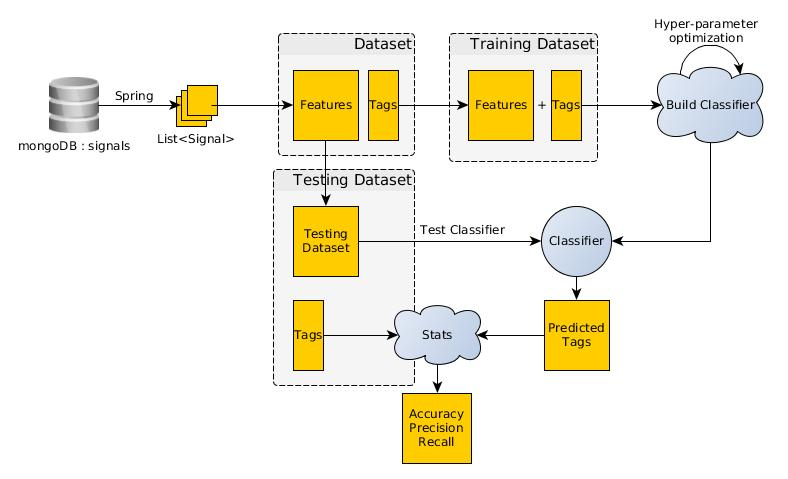
\includegraphics[width=\textwidth]{images/classifier_building.jpg}
                \caption{La construction du classifieur.}
                \label{fig:classif_building}
            \end{figure}


            \paragraph{Explication du but de chaque traitement :}
            Il faut savoir que certain traitement peuvent être réaliser seulement si, en amont, un autre traitement a été réalisé. En effet, la \textit{Lemmatization} ne peut être faite que si la chaîne de caractère a été préalablement taguée par le \textit{POS Tagger}.


            Dans un premier temps, j'ai réutilisé cette bibliothèque pour créer un classifieur binaire (2 classes) permettant de classifier les signaux relatifs aux offres d'emploi et de stage (soit le tag \textit{JOB}).

        \subsubsection{Première mise en pratique de la bibliothèque de Stanford}
                J'ai donc construis une application réalisant les actions suivantes (visible en figure \ref{fig:classif_building}) :
                \begin{itemize}
                    \item Récupérer les signaux stockés dans Mongo sous forme de liste ;
                    \item Créer un ensemble de données à partir des signaux validés manuellement ;
                    \item Diviser aléatoirement cet ensemble de données en deux ensembles (un pour entraîner le classifieur et un pour le tester) tout en gardant la proportion de chaque classe dans les deux ensembles ;
                    \item Entraîner un classifieur naïf bayésien ;
                    \item Évaluer l'erreur en généralisation et fixer les hyper-paramètres du classifier par validation croisée pendant la phase d'apprentissage ;
                    \item Évaluer la qualité du classifieur construit en calculant sa précision et son rappel sur un ensemble de données de test (qui n'ont pas \og été vu \fg jusqu'à maintenant par le classifieur).
                \end{itemize}

            \paragraph{Mes premiers choix :}
                Dans la littérature de la classification de texte, comme la détection de spam dans les emails ou l'analyse des sentiments (savoir si un texte est critique ou élogieux), il est plutôt commun de construire des classifieur naïf bayésien. Ainsi, j'ai choisi de construire un tel classifieur pour catégoriser mes signaux.\\

            J'ai choisi de créer un classifieur naïf bayésien après avoir lu les cours de l’université de Stanford sur le sujet, accessibles librement sur Internet. Ils proviennent du livre \textit{Introduction to Information Retrieval}\autocite{ir_web}.
            En parallèle, j'ai visionné sur coursera les vidéos que cette même université avait diffusé suite à un MOOC sur le \textit{Natural Language Processing}. Grâce à ces cours, j'ai pris conscience de toute l'importance du travail de prétraitement nécessaire à mettre en place, afin de bien normaliser et formater les données textuelles avant d'en faire quelque chose.\\

            Cette remarque prend tout son sens quand les données manipulées en plus d'être textuelles, ne sont pas normalisées (ou pas structurées).\\

            Dans ma formation en \textit{Natural Language Processing}, j'ai également lu les livres \textit{Natural Language Processing with Python}\autocite{nlp_p} et \textit{Python 3 Text Processing with NLTK 3 Cookbook}\autocite{nltk} , ainsi que les pages internets \textit{Introduction to Information Retrieval}\autocite{ir_web}.


            \paragraph{Le QA ou Quality Assessment :}
                L'objectif du QA est de demander la contribution d'un maximum de personnes sur une tâche de validation manuelle pénible.\\
                Durant mon stage j'ai organisé plusieurs QA pour approfondir l'ensemble des signaux d’apprentissage et de test.

            \paragraph{Proportion de signaux intéressants :}
                La quantité de signaux n'ayant pas d'intérêt, ici, est énorme (plus de 70\%). De ce fait, une pré-sélection des signaux à valider est nécessaire.\\
                Ainsi, j'ai réutilisé le premier classifieur implémenté en Python, construit sur la base des 1426 signaux. Ce classifieur a permis de classifier des signaux non validés.\\
                Ce sont ces signaux classifiés par le classifieur Python qui ont été sélectionnés pour être validés manuellement. Notamment ceux appartenant aux catégories EVENT, JOB et PRODUCT.\\
                Pour ceux appartenant aux catégories MONEY et PEOPLE, ils ont été sélectionnés pour être validés à l'aide d'expressions rationnelles pour faire ressortir des termes tels que \og levée de fonds \fg, \og chiffre d'affaire \fg, \og nommer \fg, \og nomination \fg, etc.
                De cette manière 2574 nouveaux signaux ont été validés manuellement.\\

            Au 27.07.2015, il y avait donc 4000 signaux validés manuellement par un humain :
            \begin{itemize}
                \item 488 catégorisés EVENT soit 12,2\%
                \item 258 catégorisés JOB soit 6,4\%
                \item 118 catégorisés MONEY soit 3\%
                \item 83 catégorisés PRODUCT soit 2,1\%
                \item 49 catégorisés PEOPLE soit 1,3\%
                \item 3004 validés mais considérés comme inintéressant soit 75\%
            \end{itemize}
